\section{Data replication in peer-to-peer systems}

\begin{frame}{MUTE}
    \vspace{-0.5cm}
    \begin{figure}
        \resizebox{\textwidth}{!}{
            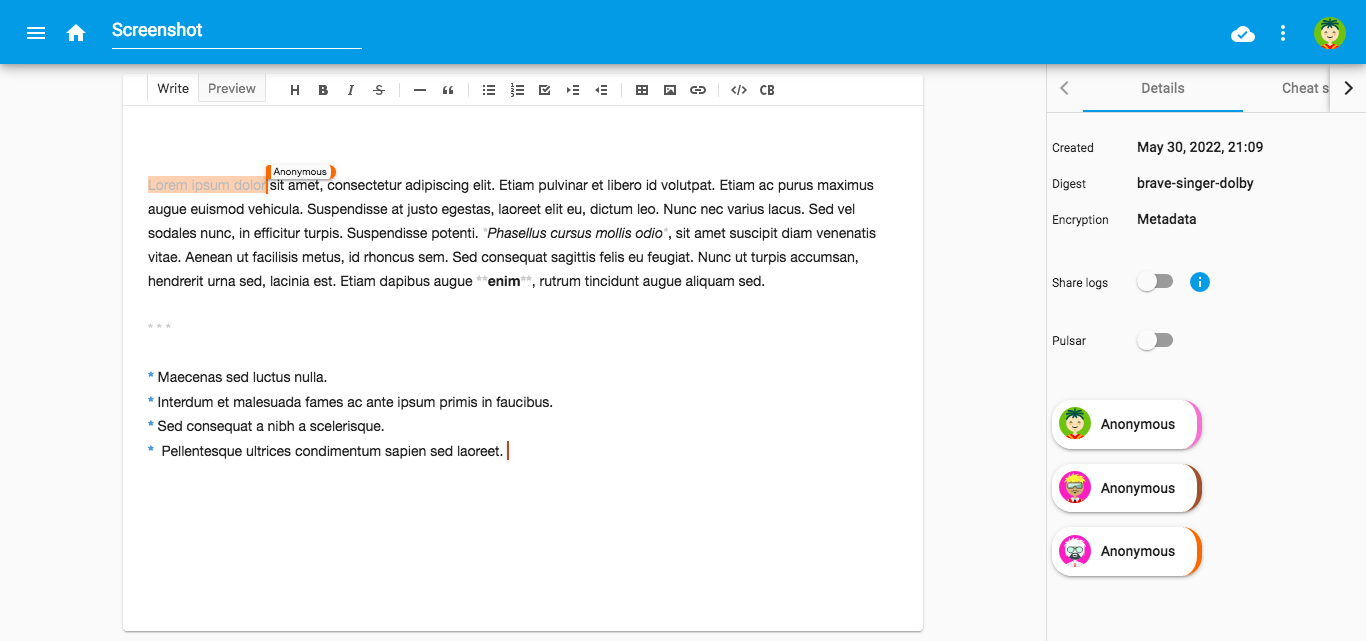
\includegraphics{img/screenshot-mute-editor.png}
        }
    \end{figure}
    \vspace{-0.5cm}
    \begin{itemize}
        \item Peer-to-Peer (P2P) application
        \item Allow to edit collaboratively text documents
        \item Ensure ownership and privacy of data
        \item Part of the Local-First Software \cite{localfirstsoftware2019} trend
    \end{itemize}
\end{frame}

\begin{frame}[fragile]{Data replication in P2P systems}
    \begin{figure}
        \resizebox{0.7 \textwidth}{!}{
            \begin{tikzpicture}
                \newcommand{\doc}{
                    \tikz{
                        \fill[scale=.15,fill=white,draw=gray,thick,solid] (0,0) -- (7,0) -- (7,8) -- (5,10) -- (0,10) -- cycle;
                    }
                }
                \newcommand{\updsquare}{
                    \tikz{
                        \fill[\colorblockone, scale=.12] (0,0) rectangle (3,3);
                    }
                }
                \newcommand{\updcircle}{
                    \tikz{
                        \fill[\colorblocktwo, scale=.07] (3,3) circle (3);
                    }
                }
                \newcommand{\updtriangle}{
                    \tikz{
                        \fill[\colorblockfive, scale=.07] (0,0) -- (6,0) -- (3,6) -- cycle;
                    }
                }
                \path
                    node[label=90:{A}] (a) {
                        \includegraphics[scale=0.4, page=5, trim=0cm 24cm 32cm 0cm, clip]{img/mute-figures.pdf}
                    }
                    +(-70:3) node[label=-90:{B}] (b) {
                        \includegraphics[scale=0.4, page=5, trim=0cm 24cm 32cm 0cm, clip]{img/mute-figures.pdf}
                    }
                    +(200:4) node[label=-90:{C}] (c) {
                        \includegraphics[scale=0.4, page=5, trim=0cm 24cm 32cm 0cm, clip]{img/mute-figures.pdf}
                    };

                \path
                    (a) node[label={[xshift=2em]0:{\doc}}] {}
                    (b) node[label={[xshift=2em]0:{\doc}}] {}
                    (c) node[label={[xshift=-2em]180:{\doc}}] {};

                \onslide<4->{
                    \path
                        (a) node[label={[xshift=3.8em]90:{\updsquare}}] {}
                        (b) node[label={[xshift=3.7em]0:{\updtriangle}}] {}
                        (c) node[label={[xshift=-4.8em]-90:{\updcircle}}] {};
                }

                \onslide<5->{
                    \draw[dotted] (a) -- (b);
                }

                \only<6>{
                    \path
                        (a) -- node[midway]{
\includegraphics[scale=0.4]{img/sync.pdf}} (b);
                }

                \onslide<7->{
                    \path
                        (a) node[label={[xshift=3.7em]0:{\updtriangle}}] {}
                        (b) node[label={[xshift=3.8em]90:{\updsquare}}] {};
                }

                \onslide<8->{
                    \draw[dotted] (a) -- (c);
                    \draw[dotted] (b) -- (c);
                }

                \only<8> {
                    \path
                        (a) -- node[midway]{
\includegraphics[scale=0.4]{img/sync.pdf}} (c)
                        (b) -- node[midway]{
\includegraphics[scale=0.4]{img/sync.pdf}} (c);
                }

                \onslide<9->{
                    \path
                        (a) node[label={[xshift=3.8em]-90:{\updcircle}}] {}
                        (b) node[label={[xshift=3.8em]-90:{\updcircle}}] {}
                        (c) node[label={[xshift=-4.8em]90:{\updsquare}}] {}
                        (c) node[label={[xshift=-4.8em]0:{\updtriangle}}] {};
                }
            \end{tikzpicture}
        }
    \end{figure}
    \vspace{-1em}
    \begin{columns}
        \hspace{0em}
        \begin{column}{0.6\textwidth}
            \begin{itemize}
                \item<2-> Nodes may be disconnected
                \item<3-> Have to be able to \alert{work without prior synchronous coordination} (i.e. consensus)
            \end{itemize}
        \end{column}
        \begin{column}{0.6\textwidth}
            \begin{itemize}
                \item<9-> Must ensure \alert{Eventual Consistency} \cite{10.1145/224057.224070}\dots
                \item<9-> \dots Despite different integration orders of updates
            \end{itemize}
        \end{column}
    \end{columns}
    \onslide<10>{
        \vspace{1em}
        \begin{center}
            \alert{Require \emph{conflict resolution mechanisms}}
        \end{center}
    }
\end{frame}

\begin{frame}[standout]
    Conflict-free Replicated Data Types (CRDTs) are a family of conflict resolution mechanisms
\end{frame}